\documentclass[
coverheight=9in,
coverwidth=6in,
spinewidth=0.4in,
bleedwidth=.125in,
marklength=0in,
markcolor=black]{bookcover}

\usepackage[T1]{fontenc}

\newbookcoverpart{pfront}{
\setpartposx{\marklength+\bleedwidth+\spinewidth+\coverwidth+10mm}
\setpartposy{\marklength+\bleedwidth+10mm}\setpartheight{\coverheight-20mm}
\setpartwidth{\coverwidth-20mm}
\settrimmedpart{0mm}{0mm}{0pt}{0pt}
}

\newbookcoverpart{pback}{
\setpartposx{\marklength+\bleedwidth+10mm}
\setpartposy{\marklength+\bleedwidth+10mm}\setpartheight{\coverheight-20mm}
\setpartwidth{\coverwidth-20mm}
\settrimmedpart{0mm}{0mm}{0pt}{0pt}
}

\begin{document}

\begin{bookcover}

\bookcovercomponent{center}{bg whole}{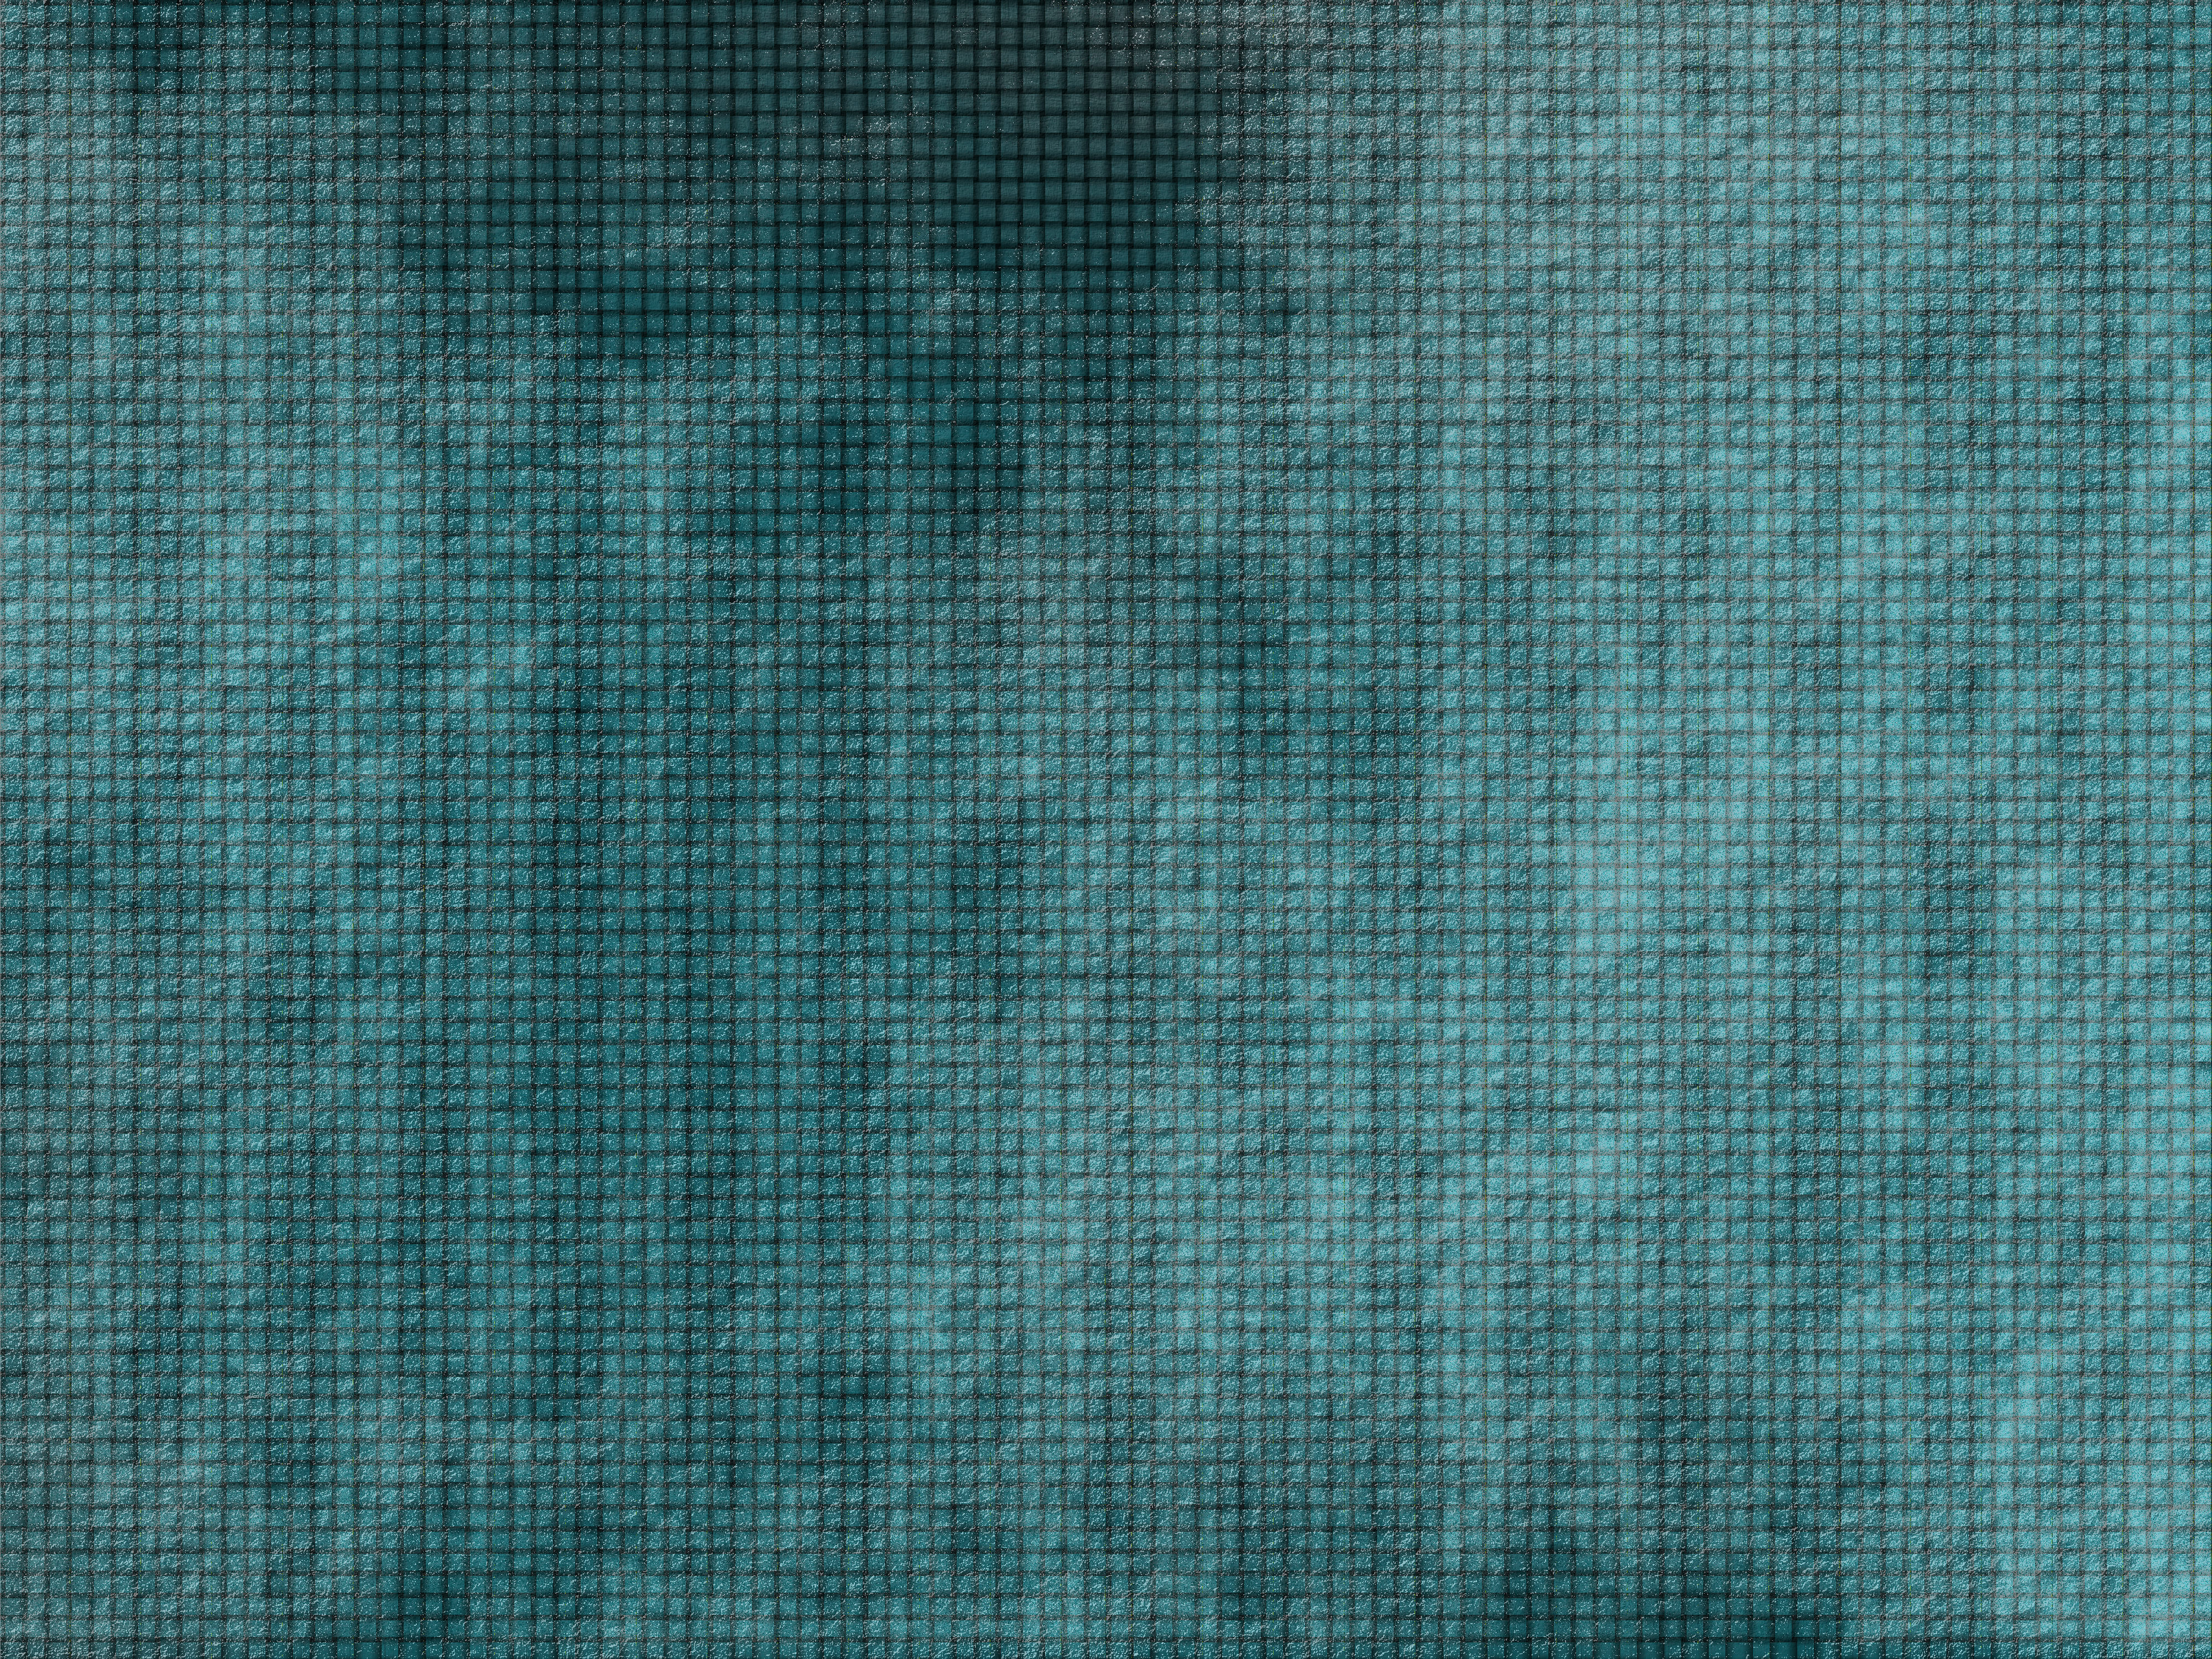
\includegraphics{fon}}

\bookcovercomponent{center}{spine}
{\rotatebox[origin=c]{-90}{
\color{white}
\fontsize{18}{25}\usefont{OT1}{lmtt}{b}{n}
PIGTIKAL
\hskip30mm
ANTON PETRUNIN
}}

\bookcovercomponent{center}{pfront}{
\begin{flushright}
{\color{white}\fontsize{75}{48}\usefont{OT1}{lmtt}{b}{n}
PIGTIKAL\\[5mm]
} 
{\color{white}\fontsize{30}{48}\usefont{OT1}{lmtt}{b}{n}Anton Petrunin}
\vfill
\includegraphics[angle=-90]{../mppics/pic-5}
\end{flushright}
}

\bookcovercomponent{center}{pfront}
{
\begin{flushleft}
\rotatebox[origin=c]{-90}{\color{white}\fontsize{28}{48}\usefont{OT1}{lmtt}{b}{n}puzzles in geometry that I know and love}
\end{flushleft}
}

\bookcovercomponent{center}{pback}{
\begin{flushleft}
\parbox{.77\textwidth}{
\color{white}\ttfamily\Large
I am collecting these problems for fun, 
but they might be used to improve 
problem-solving skills in geometry.
}
\vfill
{\color{white}\ttfamily\large  arXiv:0906.0290v14}
\\[1mm]
{\color{white}\ttfamily\large anton-petrunin.github.io/puzzles/}
\end{flushleft}
}


\end{bookcover}

\end{document}
